\newsection
\subsection{Systems}
\label{sec:systems}
\sectionauthors{Deepak Narayanan, Trevor Gale, Keshav Santhanam, Omar Khattab, Tianyi Zhang, Matei Zaharia}

\begin{figure}[!ht]
\centering
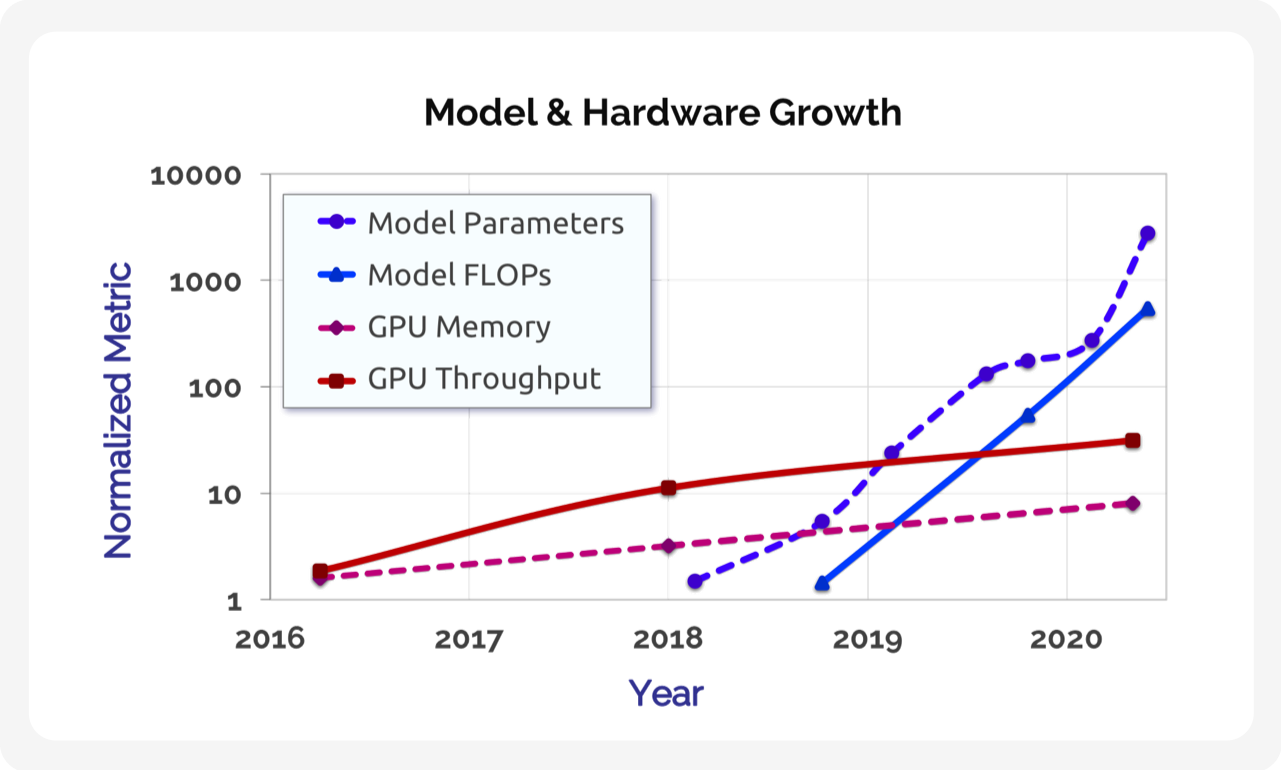
\includegraphics[width=0.7\linewidth]{technology/figures/Systems.png}
\caption{\label{fig:systems} Plot showing the growth of parameters and number of training operations (FLOPs) of transformer-based language models (shown in blue), and memory capacity and peak device throughput of NVIDIA P100, V100, and A100 GPUs (shown in red) with time. The rate of growth (slope of each line) of state-of-the-art language models (roughly $10\times$ a year) far exceeds the rate of increase in computational capacity of hardware (roughly $10\times$ in four years), motivating the need for parallelism across a large number of accelerators and co-design of algorithms, models, software, and hardware to drive further progress. Parameters and number of training operations are obtained from relevant papers~\citep{brown2020gpt3}, and memory capacities and peak throughputs are obtained from GPU specification sheets.}
\end{figure}

Computer systems are one of the largest bottlenecks to developing foundation models. Foundation models are frequently too large to fit in the main memory of a single accelerator (\eg GPU) and require an immense amount of computation to train (\eg $>1000$ petaFLOP/s-days for GPT-3~\citep{brown2020gpt3}). In addition, these models will likely get larger over time: for instance, the compute and memory requirements of state-of-the-art language models have grown by three orders of magnitude in the last three years, and are projected to continue growing far faster than hardware capabilities do (\reffig{systems}). Moreover, even once trained, these large models are expensive to perform inference with and difficult to debug, monitor, and maintain in production applications. We believe that further advances in the performance and usability of foundation models will require careful co-design across algorithms, models, software, and hardware systems, as well as new interfaces for programming and deploying ML applications. In this section, we discuss the key computer systems challenges in developing and productionizing large-scale foundation models.

\subsubsection{Improving performance through co-design} \label{sec:systems-co-design}

Today, training large-scale foundation models requires custom software systems such as Megatron and DeepSpeed~\citep{shoeybi2019megatronlm, rasley2020deepspeed}, built on top of standard frameworks like PyTorch and TensorFlow~\citep{paszke2019pytorch, abadi2016tensorflow}. These software systems rely on a number of innovations across the stack to train models efficiently at scale: new parallelization dimensions such as pipeline parallelism~\citep{huang2019gpipe, narayanan2019pipedream} that limit communication while keeping devices busy, state-sharding optimizers to reduce memory usage~\citep{rajbhandari2020zero}, just-in-time (JIT) compilers to optimize the computation graph~\citep{pytorchjit}, and optimized libraries like cuDNN and NCCL~\citep{nccl}. Megatron and DeepSpeed are efficient to a particular scale; for example, Megatron can extract up to 52\% of the theoretical peak throughput of modern hardware~ with approximately 3000 GPUs on a model with a trillion parameters~\citep{narayanan2021efficient}. However, scaling to larger models with more GPUs still is challenging, since existing parallelization strategies break down at larger GPU counts. Data parallelism is limited by the batch size~\citep{li2020pytorch}, pipeline parallelism by the number of layers in the model~\citep{huang2019gpipe, narayanan2019pipedream}, and tensor model parallelism by the number of GPUs in a single server~\citep{shoeybi2019megatronlm}.

While we will continue to realize performance gains from new hardware, growth in the resource requirements of large models far outstrips generational hardware improvements~\citep{brown2020gpt3}. To facilitate the next major leap in model capacity and to democratize the advances in model quality, it will be increasingly critical to \emph{co-design} training algorithms, models, software, and hardware, because many of the avenues to increase performance \emph{alter the semantics} of the training computation. For example, executing operations in lower precision (such as \texttt{fp16}) can help increase throughput on modern hardware (\eg the V100 and A100 GPUs have dedicated tensor core units for lower-precision matrix multiplication), but also affect the numerics of the optimization procedure~\citep{micikevicius2017mixed}. Similarly, exploiting weight sparsity can significantly improve training and inference times~\citep{Elsen_2020_CVPR, gale2020sparse} by only performing mathematical operations on the non-zeros in the model, but requires different training algorithms~\citep{jayakumar2021top, pmlr-v119-evci20a, dettmers2019sparse}. Other examples of co-design include model architectures that map more efficiently to hardware~\citep{pmlr-v97-so19a, child2019generating, wang2020linformer, lee2021fnet, kitaev2020reformer,longformer, tay2020efficient, ren2021combiner}, efficient optimizers~\citep{anil2020scalable, shazeer2018adafactor}, novel tokenization alternatives~\citep{xue2021byt5, tay2021charformer}, specially architected hardware training platforms~\cite{jouppi2017datacenter, mudigere2021high, selene}, and distributed parallelization strategies with relaxed weight update semantics~\citep{narayanan2019pipedream, narayanan2021memory}.

\paragraph{Case study: efficient knowledge representation.} As a concrete case study of successful co-design, retrieval-based models such as REALM, RAG, and ColBERT-QA~\cite{guu2020realm,lewis2020retrieval,Khattab-etal:2020:OpenQA} take a different approach to model design than simply increasing the number of model parameters. Instead of trying to accumulate \emph{implicit knowledge} from ever-larger datasets directly into a DNN model with billions of parameters, such as GPT-3, retrieval-based models store knowledge \emph{outside} the model parameters in the form of text passages, capturing knowledge within the passages with dense vector representations. These models then use scalable top-$k$ search mechanisms to extract knowledge pertinent to each input, while keeping the DNN model itself small (\refsec{modeling-memory}). This design improves computational efficiency as well as maintainability of the model in production: for example, developers can update the knowledge of the model just by replacing a text passage, without needing to retrain a large DNN.

Retrieval-based models have achieved promising initial results by leveraging several new cross-functional ideas, including backpropagating the loss through the retriever during training~\citep{guu2020realm} (which requires approximating the gradient through a knowledge store comprising millions of passages) and modeling fine-grained interactions between queries and passages~\citep{khattab2020colbert,Khattab-etal:2020:OpenQA} (which requires decomposing the computation into vector-level nearest-neighbor search operations). These techniques allow retrieval-based models to be accurate and efficient, but demand functionality not readily supported by popular ML frameworks and nearest-neighbor indexes (\eg~FAISS~\citep{johnson2019billion}). 


\subsubsection{Automated optimization}

Another important challenge in systems is to \emph{automate} the application of optimizations that straddle algorithms, models, software, and hardware. While many optimizations and parallelization strategies are complementary, identifying the most effective combination of optimizations is challenging since the joint search space grows combinatorially and optimizations interact in non-trivial ways~\citep{narayanan2021efficient}. Foundation models heighten the need for automated optimization as manual experimentation is expensive and time-consuming at the scale of thousands of GPUs.

Recent work in this area has focused on systems targeting semantics-preserving optimizations. In particular, systems have been proposed to automatically discover mathematically-equivalent graph substitutions~\citep{jia2019optimizing, wang2021pet}, facilitate the distributed execution of operator graphs through both high-level APIs and low-level compilers~\citep{rasley2020deepspeed, fairscale, jax2018github, shazeer2018mesh, lepikhin2020gshard}, and automate the selection of hybrid distribution strategies~\citep{jia2018beyond, santhanam2021distir}. These systems have helped deploy many foundation models in industry~\citep{fedus2021switch, m2m100, turingnlg}.

Unfortunately, automated optimization becomes much harder when composing semantics-altering optimizations (\refsec{systems-co-design}), as it is often unclear how to jointly model the statistical impacts  of these techniques (\eg~how many training iterations are needed to reach a specific accuracy?). We will therefore need new software tools, libraries, and compilers to automatically identify compositions of optimizations that target comprehensive metrics like time-to-accuracy~\citep{coleman2017dawnbench, mattson2020mlperf}. Building such tools will require tight collaboration between systems and machine learning experts.


\subsubsection{Execution and programming models}

The unique multi-task nature of foundation models provides an opportunity to amortize training and inference costs over many applications. In particular, paradigms such as adaptation mean more sharing across model instances. For example, two models prefix-tuned~\citep{li2021prefix} from the same pretrained model can share the same model ``stem,'' reducing the storage footprint (the shared stem only needs to be stored once), while also making it possible for execution to be shared and batched across the prefix-tuned models~\cite{shen2019nexus, narayanan2018accelerating}. Consequently, the specific adaptation mechanism used informs system optimization (\refsec{adaptation}).

It is an open question as to what programming interface should be used to specify that various adapted models are derived from the same pretrained model (\eg~models $Y$ and $Z$ are derived from the same pretrained model $X$), or that various components of two models share parameters (\eg~two models $A$ and $B$ share the same stem up to layer $i$). Ludwig~\cite{molino2019ludwig} and PyTorch's \texttt{Module} offer easy ways to compose functionality within a model, but no system today supports cross-model dependencies. Giving users the opportunity to provide annotations will allow training and inference systems to optimize and orchestrate computation more efficiently; without such annotations, systems will not have visibility into what computation and parameters can be shared across model instances. A model's ``adaptation history'' (what models is this particular model adapted from) can also be used for debugging: an adapted model's errors on particular types of inputs could originate from the pretrained model, pointing to issues in the pretraining process versus adaptation process. Frameworks like PyTorch, as well as software libraries for training foundation models such as HuggingFace Transformers~\citep{wolf2020transformers}, do not allow for fine-grained lineage information across entire model instances to be specified.

Building and maintaining a cluster of thousands of accelerators also requires tremendous effort. New training paradigms like Learning@Home~\citep{Ryabinin2020Learninghome, Diskin2021collab} explore leveraging volunteer compute over the internet to train foundation models collaboratively. Such fundamentally new execution models can decrease the cost of training for any one entity, but require collaboration across a number of different areas like security (to ensure that a malicious volunteer cannot significantly alter the training process), distributed systems (to deal with fault tolerance issues as volunteers drop), and crowdsourcing.


\subsubsection{Productionization of foundation models}

As the community continues to push the capabilities of foundation models, realizing their potential will require addressing the challenges associated with deploying these resource-intensive models in production. These challenges include performing model inference with tight latency targets, and ensuring that models and data are monitored in an automated way.

For applications with strict cost and latency constraints, model compression techniques like distillation~\citep{hinton2015distilling, li2020train, sanh2019distilbert}, quantization~\citep{polino2018model, gholami2021survey, zhou2018adaptive}, pruning~\citep{lecun1990optimal, gordon2020compressing, mccarley2019structured, wang2019structured, sajjad2020effect}, and sparsity~\citep{gale2020sparse, Elsen_2020_CVPR} could aid deployment by transforming larger models to obtain desired inference-time properties. These techniques were originally intended for smaller models (\eg BERT-L) in low-memory environments (\eg mobile phones), but are now necessary to handle the extreme scale of modern foundation models in datacenter deployments. Parallelization techniques like tensor model parallelism~\cite{shoeybi2019megatronlm}, traditionally used for training, might also be useful to reduce inference latency, and also provide additional memory capacity across GPUs to fit the model's parameters.

In addition to these practical constraints, increases in the size and complexity of foundation models and the datasets used to train them pose new challenges to model and dataset lifecycle management. Since models with a large number of parameters are hard to manually inspect by humans, we need better systems for automated dataset curation (\refsec{data}) and model quality assurance. Techniques like behavioral testing~\citep{ribeiro2020beyond} and model assertions~\citep{kang2020model} facilitate easier model maintenance in production by providing analogs to unit tests, runtime monitoring (in the form of test-time assertions), and continuous model improvement (as new inputs come in) for models deployed in end applications. These tools can help address issues of fairness and bias (\refsec{fairness}), and reduce model mispredictions.
